\vbox to \myposterheight{%
%----------------------------------------------------------------------------------------
%	OBJECTIVES
%----------------------------------------------------------------------------------------

\begin{block}{Introduction and objectives}
	
	\begin{enumerate}
		\item Ultrasound~(US) imaging uses multiple piezo-electric elements to transmit and receive acoustic pulses
		\item Time-domain beamforming techniques require sampling rates ranging from \num{3} to \num{10} times the center frequency to minimize the delay-quantization errors
		\item Such sampling rates may not be achievable in challenging environment, \textit{e.g.} portable devices
		\item We present a \textbf{compressed-sensing-based US acquisition and reconstruction approach}
	\end{enumerate}
	
\end{block}
\vfill
%----------------------------------------------------------------------------------------
%	Notations
%----------------------------------------------------------------------------------------

\begin{block}{Notations and model}
	
	\begin{columns} % Subdivide the first main column
		\begin{column}{.54\textwidth} % The first subdivided column within the first main column
			\begin{itemize}
				\item Notations:
				\begin{itemize}
					\item 1D probe composed of $N_{el}$ transducer elements located at $\bm{r}_i$
					\item $m_i\left(t\right)$ signal received at $i^{th}$ element
					\item $\psi \left(t\right)~=~\left(e \ast h_{Tx} \ast h_{Rx}\right) \left(t\right)$ elementary waveform
					\begin{itemize}
						\item $e\left(t\right)$ excitation
						\item $ h_{Tx}\left(t\right)$ impulse response in transmit
						\item  $ h_{Rx}\left(t\right)$ impulse response in receive
					\end{itemize} 
					\item Medium composed of K inhomogeneities located at $\bm{r}_k$ and with reflectivity $\gamma \left(\bm{r}_k\right)$
				\end{itemize}
			\end{itemize}
		\end{column}
		
		\begin{column}{.43\textwidth} % The second subdivided column within the first main column
			\centering
			\begin{figure}
				{\footnotesize
				\begin{tikzpicture}[%
	scale=\columnwidth/15cm,
	>={Stealth[inset=0pt]},
	thick,
	transducer/.style = {scale=\columnwidth/15cm, shape=rectangle, draw=black, fill=transducer-color, thick, minimum height=\transducerHeight cm, minimum width=\transducerWidth cm, inner sep=0pt},
	measurement/.style = {decorate, decoration=snake, color=measurement-color, thick}
	]
	% Help grid
%	\draw[help lines] (0,0) grid[step=0.5cm] (20, -15);
	
	% Transducers
	\coordinate (pos_td1) at (\transducerInitXPos, {0.5*\transducerHeight});
	\coordinate (xoff_td) at (\transducerXOffset, 0);
	
	\foreach \pt in {1,...,\transducerNumb}
		\node[transducer] (td\pt) at ($ (pos_td1) + \pt*(xoff_td) - (xoff_td) $) {};
	
	% Scatterer
	\pgfmathsetmacro{\scatPointX}{9.6} % use axes_orig
	\pgfmathsetmacro{\scatPointZ}{6.2}

	% http://tex.stackexchange.com/questions/3594/tikz-node-labels-more-below-than-below#3596
%	\node[fill, shape=circle, minimum size=0.1cm, inner sep=0cm, outer sep=0cm, color=scatterer-color, label=below:\textcolor{scatterer-color}{$\left(\vect{r}, \gamma\left(\vect{r}\right)\right)$}] (scatterer_point) at (\scatPointX, -\scatPointZ) {}; % NOT exactly 0.1cm radius..., not exactly the correct "below" distance
	\node[fill, shape=circle, minimum size=0.1cm, inner sep=0cm, outer sep=0cm, color=scatterer-color] (scatterer_point) at (\scatPointX, -\scatPointZ) {};
	\fill[color=scatterer-color] (scatterer_point) circle[radius=0.1] node[below]{$\left(\vect{r}_k, \gamma\left(\vect{r}_k\right)\right)$};
	
	% Measurements
%	\pgfmathsetmacro{\pt}{7}
%	\pgfmathsetmacro{\tdPosX}{\transducerInitXPos+(\pt-1)*\transducerXOffset}
%	\pgfmathsetmacro{\rForward}{\scatPointZ} % z
%	\pgfmathsetmacro{\rBackward}{sqrt((\scatPointX - \tdPosX)^2 + \scatPointZ^2)}
%	\pgfmathsetmacro{\rTot}{\rForward+\rBackward}
%	\pgfmathsetmacro{\tPulseCenter}{\rTot/1 - 11.5}
%	
%	\pgfmathsetmacro{\tStart}{\measurementLength - \tPulseCenter - 1/2}
%	\pgfmathsetmacro{\tEnd}{\tStart + 1}
%	\draw[domain=0:\tStart, thick, smooth, variable=\t, red] plot ({\tdPosX+0*\t}, {\t+\transducerHeight});
%	\draw[domain=0:1, thick, smooth, variable=\t, red]  plot ({\tdPosX + 0.5*(1-cos((2*pi*\t) r))*0.4*\transducerWidth*sin(3*2*pi*(\t) r)},{\transducerHeight+\tStart+\t});
%	\draw[domain=\tEnd:\measurementLength, thick, smooth, variable=\t, red] plot ({\tdPosX+0*\t}, {\t+\transducerHeight});
%	%	\node[above] at (\tdPosX, \measurementLength + \transducerHeight) {\rotatebox{90}{\textcolor{blue}{\tPulseCenter}}};
	
	\begin{scope}[on background layer]
	\foreach \pt in {1,...,\transducerNumb}
	{
		\pgfmathsetmacro{\tdPosX}{\transducerInitXPos+(\pt-1)*\transducerXOffset}
		\pgfmathsetmacro{\rForward}{\scatPointZ} % z
		\pgfmathsetmacro{\rBackward}{sqrt((\scatPointX - \tdPosX)^2 + \scatPointZ^2)}
		\pgfmathsetmacro{\rTot}{\rForward+\rBackward}
		\pgfmathsetmacro{\tPulseCenter}{\rTot/1 - 11.5}
		
		\pgfmathsetmacro{\tStart}{\measurementLength - \tPulseCenter - 1/2}
		\pgfmathsetmacro{\tEnd}{\tStart + 1}
		\draw[domain=0:\tStart, thick, smooth, variable=\t, measurement-color] plot ({\tdPosX+0*\t}, {\t+\transducerHeight});
		\draw[domain=0:1, thick, smooth, variable=\t, measurement-color]  plot ({\tdPosX + 0.5*(1-cos((2*pi*\t) r))*0.4*\transducerWidth*sin(3*2*pi*(\t) r)},{\transducerHeight+\tStart+\t});
		\draw[domain=\tEnd:\measurementLength, thick, smooth, variable=\t, measurement-color] plot ({\tdPosX+0*\t}, {\t+\transducerHeight});
%		\node[above] at (\tdPosX, \measurementLength + \transducerHeight) {\rotatebox{90}{\textcolor{blue}{\tPulseCenter}}};
		
		% Measurement label
%		\draw[] (\tdPosX, \transducerHeight) -- node[midway, sloped, below]{$m\left(\vect{r}_i, t\right)$} (\tdPosX, {\tStart+\transducerHeight});
		\ifdefstrequal{\pt}{\transducerLabeled}{%
			\fill[color=measurement-color] (\tdPosX, {\tStart+\transducerHeight}) circle[radius=0] node[below left]{\rotatebox{90}{$m_i\left( t\right)$}};
			% COULD USE \path without option for an invisible path
		}{}
		
	}
	\end{scope}
	
	% Labels for transducer and measurement
	\pgfmathsetmacro{\tdPosX}{\transducerInitXPos+(\transducerLabeled-1)*\transducerXOffset}
	\node[above] at (td\transducerLabeled) {$\vect{r}_i$};
%	\node[above] at (\tdPosX, \measurementLength + \transducerHeight) {\rotatebox{90}{\textcolor{measurement-color}{$m\left(\vect{r}_i, t\right)$}}};
	
	
	% Axes
	\pgfmathsetmacro{\vertAxisX}{\transducerInitXPos - \axesOffset}
	\pgfmathsetmacro{\transducerLength}{(\transducerNumb-1)*\transducerXOffset}
	\coordinate (axes_orig) at (\vertAxisX, 0);
	\coordinate (x_axis_end) at ({\transducerInitXPos + \transducerLength + \axesOffset}, 0);
	\coordinate (z_axis_end) at (\vertAxisX, {-\scatPointZ - \axesOffset});
	\coordinate (t_axis_start) at (\vertAxisX, \transducerHeight + \measurementLength);
	\coordinate (t_axis_end) at (\vertAxisX, \transducerHeight + \axesOffset);
	
	\draw[<->] (x_axis_end) node[right] {$x$} -- (axes_orig) -- (z_axis_end) node[below] {$z$};
	\draw[->] (t_axis_start) -- (t_axis_end) node[below] {$t$};

	% Plane wave: Wavefront and transmit time of flight
	\pgfmathsetmacro{\thetaPW}{15} % degree
	\pgfmathsetmacro{\thetaLabXOffset}{2.2}
	\pgfmathsetmacro{\PWaveFrontStartX}{\transducerInitXPos}
	\pgfmathsetmacro{\PWaveFrontStartZ}{\transducerHeight}
	\pgfmathsetmacro{\PWaveFrontEndX}{\transducerInitXPos+\transducerLength}
	\pgfmathsetmacro{\PWaveFrontEndZ}{\transducerHeight+sin(\thetaPW)*\transducerLength}
	\coordinate (pw_wavefront_start) at (\PWaveFrontStartX, \PWaveFrontStartZ);
	\coordinate (pw_wavefront_end) at (\PWaveFrontEndX, \PWaveFrontEndZ);
	\coordinate (pw_wavefront_scat_proj) at ($(pw_wavefront_start)!(scatterer_point)!(pw_wavefront_end)$);
	
	%	Transmit wavefront
	\begin{scope}[on background layer]
		\draw[dashed, wavefront-color, thick, name path=pw_wavefront_path] (pw_wavefront_start) -- (pw_wavefront_end);
		%TODO: use clip on an extended path line
	\end{scope}
%	%		Angle
%	\begin{scope}[on background layer]
%		\draw[wavefront-color, thin] ({\PWaveFrontStartX+\thetaLabXOffset},{\PWaveFrontStartZ}) arc[start angle=0, end angle=\thetaPW, radius=\thetaLabXOffset] node[midway, right]{$\theta$};
%	\end{scope}
	
	% 		Wavefront label
	\path[name path=data_right_limit_path] ({\transducerInitXPos+\transducerLength}, 0) -- ({\transducerInitXPos+\transducerLength}, {\transducerHeight+\measurementLength});
	\fill[name intersections={of=pw_wavefront_path and data_right_limit_path, by = pw_wavefront_label_point}] (pw_wavefront_label_point) circle[radius=0] node[right, align=center, wavefront-color]{}; % specificying the key align= allows to add newlines
	
	%	Transmit time of flight
	\draw[->, wavefront-color] (pw_wavefront_scat_proj) -- node[midway, sloped, below] {$t_{Tx}\left(\vect{r}\right)$} (scatterer_point);
	
%	% Diverging wave: Wavefront and transmit time of flight
%	\pgfmathsetmacro{\DWVirtualPointX}{\transducerInitXPos + 3}
%	\pgfmathsetmacro{\DWVirtualPointZ}{1.2*\measurementLength + \transducerHeight}
%	\pgfmathsetmacro{\DWBetaAngleRadius}{0.35cm}
%	
%	%	Virtual point
%	\node[fill, shape=circle, minimum size=0.1cm, inner sep=0cm, outer sep=0cm, color=wavefront-color] (dw_virtual_point) at (\DWVirtualPointX, \DWVirtualPointZ) {};
%	\fill[color=wavefront-color] (dw_virtual_point) circle[radius=0] node[above]{$\vect{r}_n$};
%	
%	%	Wavefront
%	\begin{scope}[on background layer]
%%		\clip (\transducerInitXPos, \transducerHeight) rectangle ({\transducerInitXPos+\transducerLength}, {\transducerHeight, \measurementLength});
%		\begin{scope} % just for the clip
%			\clip (\transducerInitXPos, \transducerHeight) rectangle ({\transducerInitXPos+\transducerLength}, {\transducerHeight+\measurementLength});
%%		\path[draw, thick, wavefront-color, name path=dw_wavefront_path] (dw_virtual_point) circle [radius={\DWVirtualPointZ-\transducerHeight}];
%			\draw[dashed, thick, wavefront-color, name path=dw_wavefront_path] (dw_virtual_point) circle [radius={\DWVirtualPointZ-\transducerHeight}];
%		\end{scope}
%	\end{scope}
%	
%	% 		Wavefront label
%	\path[name path=data_right_limit_path] ({\transducerInitXPos+\transducerLength}, 0) -- ({\transducerInitXPos+\transducerLength}, {\transducerHeight+\measurementLength});
%	\fill[name intersections={of=dw_wavefront_path and data_right_limit_path, by = dw_wavefront_label_point}] (dw_wavefront_label_point) circle[radius=0] node[right, align=center, wavefront-color]{``wavefront''}; % specificying the key align= allows to add newlines
%	
%	%	Intersection on the circular wavefront
%	\path[name path=dw_virtual_point_to_scatterer] (dw_virtual_point) -- (scatterer_point);
%	
%	% 	Transmit time of flight
%	\fill[name intersections={of=dw_wavefront_path and dw_virtual_point_to_scatterer, by = dw_point_on_wavefront}] (dw_point_on_wavefront) circle[radius=0];
%%	\draw[-, wavefront-color] [name intersections={of=dw_wavefront_path and dw_virtual_point_to_scatterer, by = dw_point_on_wavefront}] (dw_virtual_point) -- (dw_point_on_wavefront);
%	\draw[dotted, wavefront-color] (dw_virtual_point) -- (dw_point_on_wavefront);
%	\draw[->, wavefront-color](dw_point_on_wavefront) -- node[midway, sloped, below] {$t_{Tx}\left(\vect{r}\right)$} (scatterer_point);
%	\begin{scope}[on background layer]
%		\path[name path=transducer_height_path] (\vertAxisX, \transducerHeight) -- ({\transducerInitXPos+\transducerLength+\axesOffset}, \transducerHeight);
%		%	Angle
%		\fill[red, name intersections={of=transducer_height_path and dw_virtual_point_to_scatterer, by = dw_beta_base_point}] (dw_beta_base_point) circle[radius=0cm];
%		\pic[pic text=$\beta$, draw, wavefront-color, thin, angle radius=\DWBetaAngleRadius, angle eccentricity=1.4] {angle= dw_virtual_point--dw_beta_base_point--td1};
%	\end{scope}
%
%	
	% Receive time for flight
	\draw[->, wavefront-color] (scatterer_point) -- node[midway, sloped, below] {$\frac{\vect{r}-\vect{r}_i}{c}$} (td\transducerLabeled.south);
%	
%	% 1-D conic (ellipse)
%	\coordinate (dw_ellipse_focus1) at (dw_virtual_point);
%	\coordinate (dw_ellipse_focus2) at (td\transducerLabeled);
%	\begin{scope} % just for the clip
%		\clip (\transducerInitXPos, 0) rectangle ({\transducerInitXPos+\transducerLength}, -\domainZMax);
%		\ellipsebyfoci{draw, conic-color, name path=dw_conic_path}{dw_ellipse_focus1}{dw_ellipse_focus2}{16.5}
%	\end{scope}
%	%	Conic label
%	\newcommand*{\conicTextLabel}{``ellipse''}
%	\newcommand*{\conicMathLabel}{$\left[
%		x\left(\alpha\right), z\left(\alpha\right)\right]^T$}
%	\pgfmathsetmacro{\vertGridX}{\transducerInitXPos+9*\transducerXOffset}
%	\path[name path=domain_vert_path] (\vertGridX, 0) -- (\vertGridX, -\domainZMax);
%	\fill[name intersections={of=dw_conic_path and domain_vert_path, by = dw_conic_label_point}] (dw_conic_label_point) circle[radius=0] node[right, align=center, conic-color]{\conicTextLabel}; % specificying the key align= allows to add newlines
%	
%	% Insonified domain (i.e. Grid)
%	% http://tex.stackexchange.com/questions/45808/tikz-grid-lines
%	\begin{scope}[on background layer]
%		\draw[step=1, very thin, color=domain-color] (\domainXMin, -\domainZMin) grid (\domainXMax, -\domainZMax);
%	\end{scope}
%	
%	% 	Discretization
%	\pgfmathsetmacro{\discretizedPointLabeledNumb}{3}
%%	\newcommand*{\discretizedPointMathLabel}{$\left[
%%		x\left(\alpha^p\right), z\left(\alpha^p\right)\right]^T$}
%	\newcommand*{\discretizedPointMathLabel}{$\vect{r}\left(\alpha^p\right)$}
%	%		TODO: set a gridNumb
%	\foreach \gridVert in {1,...,\transducerNumb}
%	{
%		\pgfmathsetmacro{\vertGridX}{\domainXMin+(\gridVert-1)*\domainDxOffset}
%		\path[name path=domain_vert_path] (\vertGridX, -\domainZMin) -- (\vertGridX, -\domainZMax);
%		\fill[name intersections={of=dw_conic_path and domain_vert_path, by = discretized_conic_point}] (discretized_conic_point) circle[radius=0.1];
%		
%		\ifdefstrequal{\gridVert}{\discretizedPointLabeledNumb}{%
%			\fill (discretized_conic_point) circle[radius=0] node[above right]{\discretizedPointMathLabel};
%			% COULD USE \path without option for an invisible path
%		}{}
%	}
%	
%	%	Grid spacing
%	\newcommand*{\spacingLabelOffset}{7pt}
%	\pgfmathsetmacro{\domainDxIndexX}{8} % 1 - 10
%	\pgfmathsetmacro{\domainDxIndexZ}{8} % 1 - 8
%	\pgfmathsetmacro{\domainDzIndexX}{10} % 1 - 10
%	\pgfmathsetmacro{\domainDzIndexZ}{6} % 1 - 8
%	\pgfmathsetmacro{\domainDxOneX}{\domainXMin+(\domainDxIndexX-1)*\domainDxOffset}
%	\pgfmathsetmacro{\domainDxTwoX}{\domainXMin+(\domainDxIndexX)*\domainDxOffset}
%	\pgfmathsetmacro{\domainDxOneZ}{-\domainZMin-(\domainDxIndexZ-1)*\domainDzOffset}
%	\pgfmathsetmacro{\domainDxTwoZ}{-\domainZMin-(\domainDxIndexZ-1)*\domainDzOffset}
%	\pgfmathsetmacro{\domainDzOneX}{\domainXMin+(\domainDzIndexX-1)*\domainDzOffset}
%	\pgfmathsetmacro{\domainDzTwoX}{\domainXMin+(\domainDzIndexX-1)*\domainDzOffset}
%	\pgfmathsetmacro{\domainDzOneZ}{-\domainZMin-(\domainDzIndexZ-1)*\domainDzOffset}
%	\pgfmathsetmacro{\domainDzTwoZ}{-\domainZMin-(\domainDzIndexZ)*\domainDzOffset}
%%	\fill[red] (\domainDxOneX, \domainDxOneZ) circle[radius=0.1];
%%	\fill[blue] (\domainDxTwoX, \domainDxTwoZ) circle[radius=0.1];
%%	\fill[red] (\domainDzOneX, \domainDzOneZ) circle[radius=0.1];
%%	\fill[blue] (\domainDzTwoX, \domainDzTwoZ) circle[radius=0.1];
%	\coordinate (domain_dx_one) at (\domainDxOneX, \domainDxOneZ);
%	\coordinate (domain_dx_two) at (\domainDxTwoX, \domainDxTwoZ);
%	\coordinate (domain_dz_one) at (\domainDzOneX, \domainDzOneZ);
%	\coordinate (domain_dz_two) at (\domainDzTwoX, \domainDzTwoZ);
%	\draw[|-|, thin] ($ (domain_dx_one) - (0, \spacingLabelOffset) $) -- node[below] {$\Delta x$} ($ (domain_dx_two) - (0, \spacingLabelOffset) $);
%	\draw[|-|, thin] ($ (domain_dz_two) + (\spacingLabelOffset, 0) $) -- node[midway, sloped, below] {$\Delta z$} ($ (domain_dz_one) + (\spacingLabelOffset, 0) $);
%	
%	%	Inter-element spacing
%	\pgfmathsetmacro{\transducerDxiOne}{2}
%	\pgfmathsetmacro{\transducerDxiTwo}{3}
%	\draw[|-|, thin] ($ (td\transducerDxiOne.south) - (0, \spacingLabelOffset) $) -- node[below] {$\Delta x_i$} ($ (td\transducerDxiTwo.south) - (0, \spacingLabelOffset) $);
%	
%	
	\end{tikzpicture}}
				%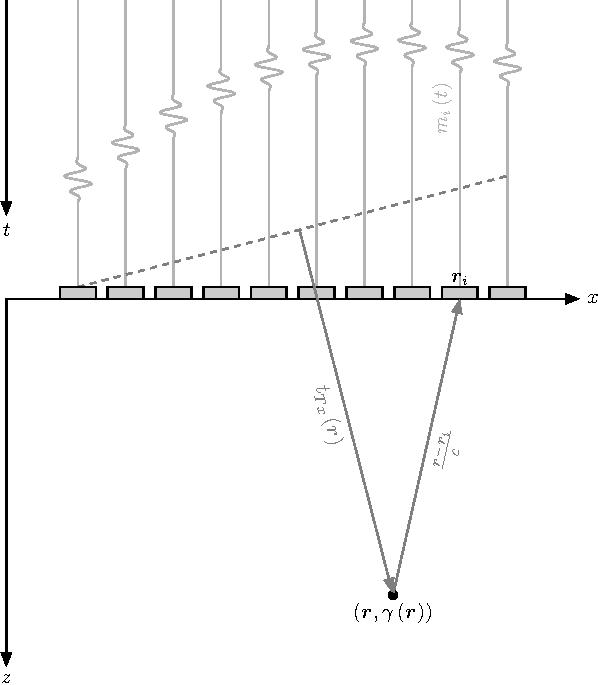
\includegraphics[width=0.9\linewidth]{tikz_SPARS-crop.pdf}
				\caption{Standard setting for US imaging}
			\end{figure}
		\end{column}
	\end{columns} % End of the subdivision
	
	\begin{itemize}
		\item The signals received at each element follow a \textbf{stream of pulses} model and can be written as:
		\begin{equation*}
		m_i\left(t\right)~=~\sum_{k=1}^{K} a_{ik} \psi \left(t - t_{k}\right)
		\end{equation*}
		with $\left(a_{ik}, t_{k}\right)_{k=1}^K$ amplitudes and times-of-arrival of the $K$ echo-pulses to the $i^{th}$ transducer-element
		\item The $N_t$ discretized samples obtained by sampling $m_i\left(t\right)$ at a frequency $f_s$ \textbf{obey a $K$-sparse synthesis model} in a dictionary $\Psi \in \mathbb{R}^{N_t \times N_t}$ made of all the shifted replicas of the pulse~\cite{naini2009}:
		\begin{equation*}
			\bm{m}_i = \Psi \bm{a}_i, \textnormal{ with } \| \bm{a}_i\|_0 = K
		\end{equation*}
	\end{itemize}
	
\end{block}
\vfill 
%----------------------------------------------------------------------------------------
%	METHODS
%----------------------------------------------------------------------------------------

\begin{block}{The proposed acquisition scheme: US compressive multiplexer}
	\begin{column}{.54\textwidth} % The first subdivided column within the first main column
		\begin{itemize}
			\item \textbf{CMUX}~\cite{kim2012}: Signals from M sensors are modulated and summed:
			\begin{equation*}
			y \left(t\right)~=~ \sum_{i=1}^{M} p_i \left(t\right) m_i \left(t\right)
			\end{equation*}
			where $p_i\left(t\right)$ is a chipping sequence drawn from a Rademacher distribution
			\item Signal $y \left(t\right)$ sampled at $f_s$ leading to a compression by a factor of M
			\item \textbf{US-CMUX}: Use L CMUX each of which grouping M sensors and sharing the same chipping sequences to perform signal acquisition
			\begin{equation*}
				\mathsf{Y} = \left[\bm{y_1}, ..., \bm{y_L}\right] \in \mathbb{R}^{N_t \times L}
			\end{equation*}
			\item Compression by a factor of M compared to standard US devices
			\item Can be achieved using mixed signal blocks~\cite{kim2012}
		\end{itemize}
	\end{column}
	\begin{column}{.43\textwidth}
		\begin{figure}[htb]
			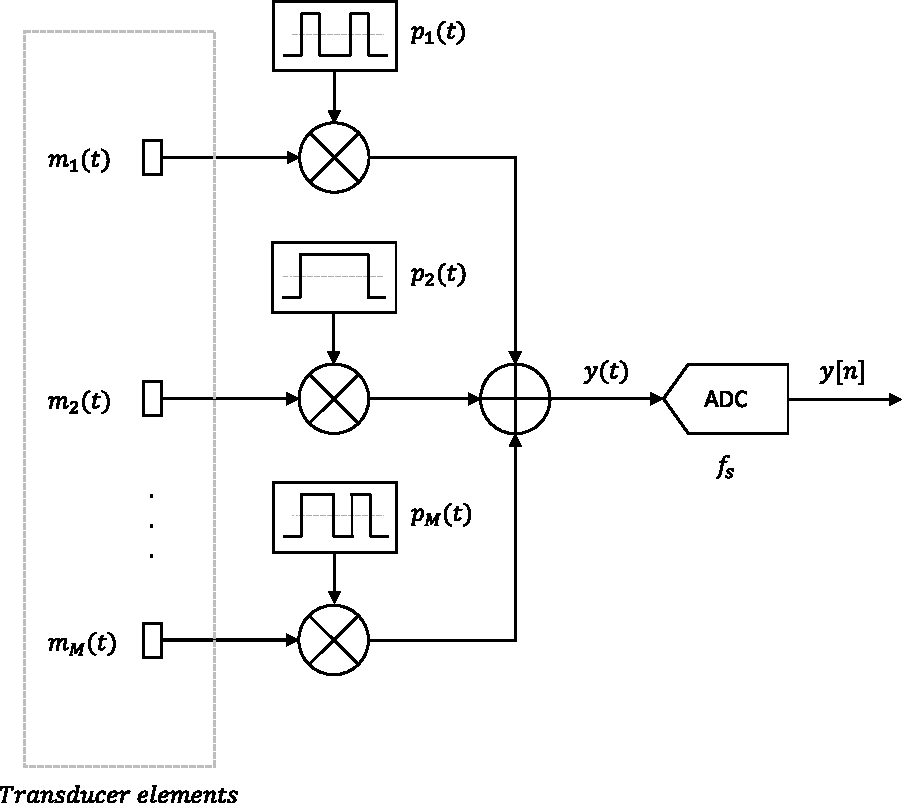
\includegraphics[width=0.8\linewidth]{figures/CMUX.pdf}
			\caption{CMUX architecture}
			\label{fig_CMUX}
		\end{figure}
	\begin{figure}[htb]
		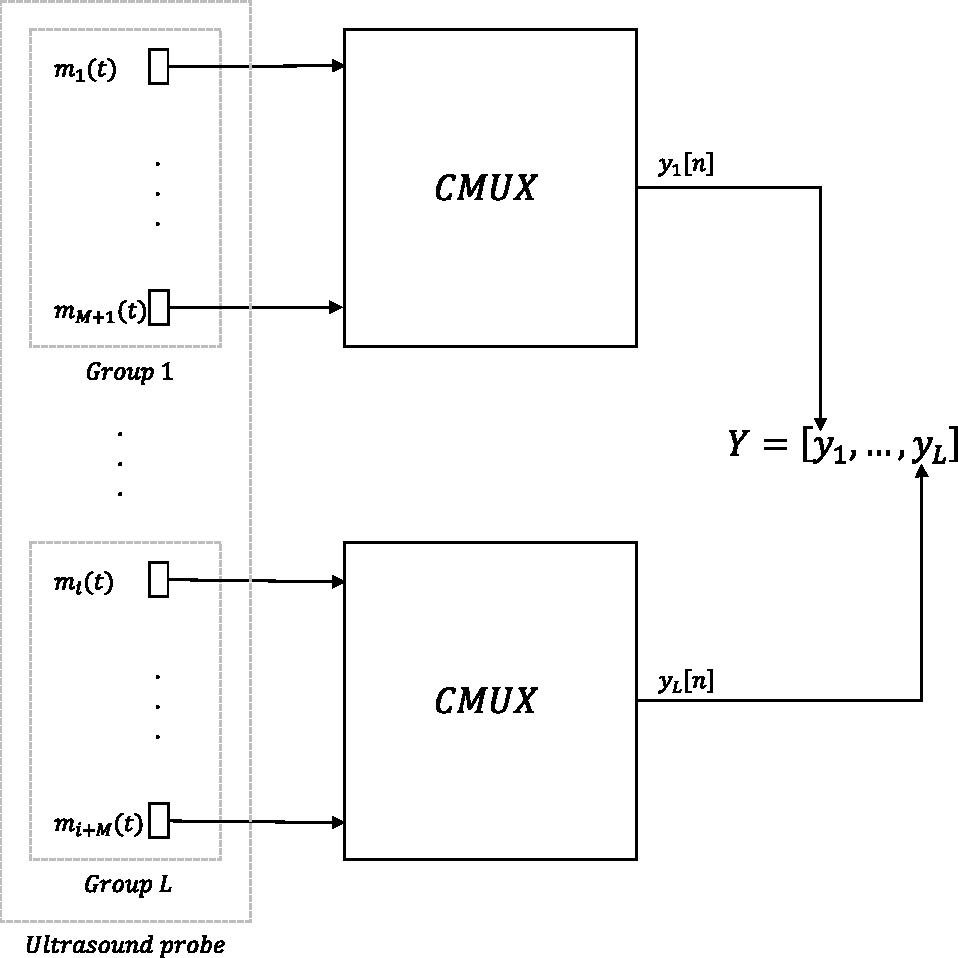
\includegraphics[width=0.8\linewidth]{figures/USCMUX.pdf}
		\caption{US-CMUX architecture}
		\label{fig_USCMUX}
	\end{figure}
	\end{column}
	
\end{block}
\vfill
%----------------------------------------------------------------------------------------
%	US image reconstruction
%----------------------------------------------------------------------------------------

\begin{block}{Proposed reconstruction algorithm}
	\begin{itemize}
		\item $\ell_{11}$-minimization problem is solved:
		\begin{equation*}
		\min_{\bar{\mathsf{A}} \in \mathbb{R}^{MN_t \times L}} \lVert \bar{\mathsf{A}} \lVert_{11}
		\textnormal{ subject to } \| \mathsf{Y}- \Psi_{P}\bar{\mathsf{A}}\|_F\leq\epsilon
		\end{equation*}
		$\Psi_{P}~=~\left[\Psi_{p1}, ..., \Psi_{pM}\right] \in \mathbb{R}^{N_t \times M N_t}$, $\Psi_{pi}~=~\left[\bm{p}_i \otimes \Psi_1, ..., \bm{p}_i \otimes \Psi_{N_t}\right] \in \mathbb{R}^{N_t \times N_t}$ 
		\begin{equation*}
		\mathsf{A}=
		\begin{bmatrix}
		\bm{a}_1 & \bm{a}_{M+1} & \dotsb & \bm{a}_{N_{el}-M+1}\\
		\vdots & \vdots & & \vdots \\
		\bm{a}_M & \bm{a}_{2M} & \dotsb &\bm{a}_{N_{el}} \\
		\end{bmatrix}
		\end{equation*}
		\item Solved with primal dual forward backward algorithm~\cite{combettes2014} 
	\end{itemize}
\end{block}
%----------------------------------------------------------------------------------------
}%